In this chapter, we will introduce the background, vulnerabilities, and threats of Industrial Control Systems (ICS) and the Modbus TCP protocol in more detail. In addition, we will also introduce the technologies and frameworks used in our monitoring system, including Suricata, Graylog (SIEM), the ICS Cyber Kill Chain, and the ISA/IEC 62443-3-3 standard.

\section{{Industrial Control Systems (ICS) Security} }
In modern critical infrastructure protection, understanding the fundamental differences between OT and IT networks is necessary to avoid causing unintended operational disruptions. Therefore, recognizing the unique architecture of ICS is the first step in designing appropriate defense mechanisms.

\subsection{OT vs. IT Network Characteristics}
According to the NIST SP 800-82 guide, IT networks prioritize data confidentiality, whereas OT networks highly value system availability and personnel safety \cite{ref_report13}. This fundamental difference makes it difficult to directly apply traditional IT security tools to ICS environments. Unlike IT networks where powerful servers and PCs are the primary endpoints, OT networks are centered around Programmable Logic Controllers (PLCs) and field devices. PLCs are resource-constrained devices designed for strict real-time processing, long-term stability, and high availability, typically operating for decades without hardware upgrades. Due to these computing constraints and operational continuity requirements, modern IT security mechanisms—such as frequent system patching, heavy encryption algorithms, and active anti-virus scanning—are often impractical for PLC environments.

Furthermore, a critical yet frequently overlooked distinction in OT threat modeling lies in the network topology and attack vectors. While traditional IT security breaches usually involve attacks spanning across multiple routed subnets, malicious activities in OT environments predominantly manifest as intra-subnet attacks occurring within a single local area network (LAN) \cite{ref_report13}. Because legacy industrial control subnets—particularly at Level 1 and Level 2—were historically designed under the assumption of absolute physical isolation, they lack basic segment-level access control and cryptographic authentication. Consequently, once an attacker successfully infiltrates the local subnet, they face minimal technical barriers; they can passively sniff unencrypted broadcast traffic or execute address spoofing (such as ARP poisoning and IP spoofing) to impersonate legitimate master stations (HMIs) or slave devices (PLCs) \cite{ref_report13}. This lack of boundary defense within the same subnet highlights the extreme structural vulnerability of industrial network architectures.

To define the hierarchical structure of ICS, isolate these vulnerable edge devices, and establish network segmentation, the Purdue Enterprise Reference Architecture (PERA) is widely adopted. This research follows an enhanced PERA model that incorporates an Industrial Demilitarized Zone (IDMZ) at Level 3.5. Notably, Level 0 to Level 2—encompassing physical processes, local controllers (such as PLCs), and supervisory systems—constitutes the primary domain for Modbus communications analyzed in this study. The functional roles of each level in this architecture are summarized below:
\newpage
\begin{itemize}
    \item 
    \textbf{Level 5 (Enterprise Networks):} Hosts corporate IT infrastructure and external services (e.g., Enterprise Firewalls, Mail and Web Servers).
    \item 
    \textbf{Level 4 (Business Networks):} Manages internal administrative operations via DNS, Business Servers, and Enterprise Desktops.
    \item 
    \textbf{Level 3.5 (IT/OT DMZ):} Acts as a critical security perimeter preventing direct access between IT and OT, utilizing IDMZ Firewalls and Jump Servers.
    \item 
    \textbf{Level 3 (Operations Systems):} Centralizes plant-wide management through HMIs, Historians, and Application/Database Servers.
    \item 
    \textbf{Level 2 (Supervisory Control):} Provides localized process monitoring via SCADA and Local HMIs. Notably, Levels 0 to 2 constitute the primary domain for Modbus communications analyzed in this research.
    \item 
    \textbf{Level 1 (Process Control):} Executes real-time automated control using intelligent devices like PLCs, RTUs, and DCS Controllers.
    \item 
    \textbf{Level 0 (Physical Process):} Comprises physical field devices, such as sensors, actuators, and pumps, for direct environmental interaction.
\end{itemize}
\newpage
As IT and OT networks rapidly converge, these traditional boundaries blur, requiring a robust defense-in-depth strategy \cite{ref_report13}. Figure~\ref{fig:Figure_2.1.jpg} illustrates the hierarchical boundaries based on this model.

\begin{figure}[htbp]
\centering
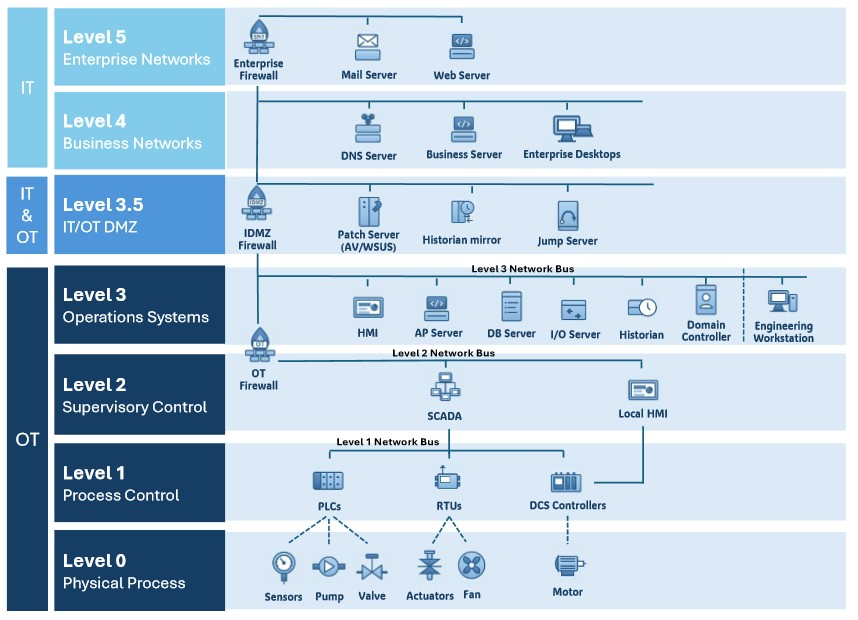
\includegraphics[width=15cm]{figure/Figure_2.1.jpg}
\caption{Purdue Enterprise Reference Architecture} \label{fig:Figure_2.1.jpg}
\end{figure}

\newpage
\subsection{Modbus TCP Protocol Architecture and Exception Response}
Modbus TCP is a commonly used communication protocol in industrial control systems (ICS). In the Purdue Enterprise Reference Architecture (PERA), it is often used for communication between Level 2, the Supervisory Control Level, and Level 1, the Process Control Level. Through Modbus TCP, systems such as SCADA or HMI can exchange data with PLCs and RTUs, including reading device status, collecting sensor values, and sending control commands. Since Modbus TCP is simple, easy to implement, and highly compatible with industrial devices, it is still widely used in many industrial environments today. The protocol usually communicates through TCP Port 502.

As shown in Figure (Figure~\ref{fig:Figure_2.2.jpg}), a Modbus TCP packet is mainly composed of an Application Data Unit (ADU), which includes the MBAP Header and the Protocol Data Unit (PDU). The MBAP Header is 7 bytes long and contains four fields: Transaction Identifier, Protocol Identifier, Length, and Unit Identifier. These fields are used to identify packets, indicate message length, and match requests with responses. In normal Modbus TCP communication, the Protocol Identifier should be 0x0000. Therefore, if this field contains an unexpected value, it may indicate that the packet format is abnormal or does not follow the standard Modbus TCP structure.

The PDU contains the Function Code and the Data field. The Function Code indicates the operation requested by the client, such as reading coils, reading registers, writing values, or executing diagnostic functions. The Data field carries the information required for that operation, such as the starting address, data quantity, written value, diagnostic sub-function, or exception code. Since these fields describe the operation and meaning of a Modbus TCP packet, the MBAP Header and PDU structure provide an important basis for understanding Modbus TCP communication.

\begin{figure}[htbp]
\centering
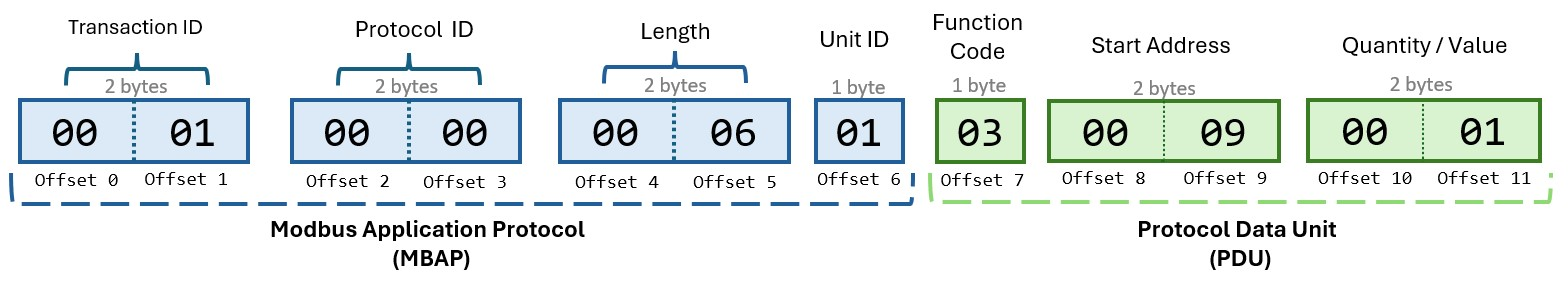
\includegraphics[width=14.5cm]{figure/Figure_2.2.jpg}
\caption{Modbus TCP Application Data Unit (ADU) Frame Structure} \label{fig:Figure_2.2.jpg}
\end{figure}

\newpage

Modbus defines four main data models: Coils, Discrete Inputs, Input Registers, and Holding Registers. These data models differ in their access permissions, data sizes, and meanings in industrial control processes. Coils and Holding Registers can be both read and written. Therefore, if they are modified without authorization, the state of field devices or process parameters may be affected directly. In contrast, Discrete Inputs and Input Registers are usually read-only and are mainly used to report digital states or analog measurement values. Table \ref{tab:modbus_data_model} summarizes the common access types, Function Codes, related Level 0 devices, and characteristics of these four data models.

\begin{table}[htbp]
\caption{Modbus Data Models and Their Characteristics}
\centering
\renewcommand{\arraystretch}{1.4}
\begin{tabularx}{\textwidth}{@{} p{1.5cm} p{1.4cm} p{1.9cm} p{3.1cm} X @{}}
\toprule
\textbf{Data Model} &
\textbf{Access} &
\textbf{Common FCs} &
\textbf{Level~0 \newline Devices} &
\textbf{Characteristics (Size)} \\
\midrule

Coils
  & Read/Write
  & Read: 01 \newline Write: \newline05、15
  & Pump, Valve
  & \textbf{1-bit.} Controls physical equipment
    (e.g.\ Coil~0 = Start Pump, Coil~1 = Open Valve). \\
\addlinespace

Discrete Inputs
  & Read Only
  & Read: 02
  & Limit Switch, Emergency Stop, Digital Sensor
  & \textbf{1-bit.} Digital sensor/switch status
    (e.g.\ Discrete Input~0 = Pump Running). \\
\addlinespace

Input \newline Registers
  & Read Only
  & Read: 04
  & Temperature Sensor, \newline Pressure \newline Transmitter
  & \textbf{16-bit.} Analog values.
    (e.g.\ Input Register~0 = Current Temperature). \\
\addlinespace

Holding Registers
  & Read/Write
  & Read : 03\newline Write: \newline06、16
  & Setpoint Controller, PID Parameter, Configuration Register
  & \textbf{16-bit.} Most commonly attacked target in ICS
    (e.g.\ Holding Register~1 = Speed Setpoint). \\

\bottomrule
\end{tabularx}

\label{tab:modbus_data_model}
\end{table}

\newpage
From a security perspective, read Function Codes such as FC01 to FC04 are mainly used for monitoring and data collection, while write Function Codes such as FC05, FC06, FC15, FC16, FC22, and FC23 can directly modify Coils or Holding Registers. Therefore, unauthorized or abnormal write operations may affect device states, process parameters, or control logic. It should also be noted that Table 2.1 only lists common Function Codes related to the four data models. Other Function Codes, such as FC08 Diagnostics and FC43 Encapsulated Interface Transport, are not directly mapped to a specific data model but are still part of the fixed operation set defined by the Modbus standard.

In addition to normal responses, Modbus TCP also defines an Exception Response mechanism. When a server or PLC cannot process a client request, it returns an Exception Response by adding 0x800 to the original Function Code and placing an Exception Code in the Data field. For example, if an FC03 request cannot be processed, the response Function Code becomes 0x830, and the following Exception Code explains the reason for the failure. Although a single Exception Response does not necessarily indicate an attack, frequent exceptions or exceptions appearing together with abnormal Function Codes, invalid addresses, or scanning behavior may indicate protocol probing, address enumeration, or fuzzing attempts.

Common Modbus Exception Codes are shown in Table Table \ref{tab:modbus_exception}.
\begin{table}[htbp]
\caption{Modbus Exception Codes and Security Implications in ICS}
\centering
\small
\renewcommand{\arraystretch}{1.25}
\setlength{\tabcolsep}{4pt}
\begin{tabularx}{\textwidth}{@{} p{1.0cm} p{3.6cm} X @{}}
\toprule
\textbf{Code} & \textbf{Name} & \textbf{Operational Meaning} \\
\midrule

0x01 & Illegal Function &
The requested Function Code is not supported or allowed by the server. It may indicate misconfiguration, probing, or fuzzing. \\
\addlinespace

0x02 & Illegal Data Address &
The requested Coil or Register address is invalid or not accessible. It may indicate address enumeration or unauthorized access attempts. \\
\addlinespace

0x03 & Illegal Data Value &
The request contains a value or parameter outside the acceptable range. It may affect control logic if related to write operations. \\
\addlinespace

0x04 & Slave Device Failure &
An error occurs while the PLC or server processes the request. It may reflect an abnormal device condition. \\
\addlinespace

0x05 & Acknowledge &
The request has been accepted but requires more processing time. It is usually related to long-duration operations. \\
\addlinespace

0x06 & Slave Device Busy &
The device is temporarily busy. Frequent occurrences may indicate excessive requests or possible DoS pressure. \\
\addlinespace

0x07 & Negative \newline Acknowledge &
The device cannot complete the requested program or diagnostic operation. \\
\addlinespace

0x08 & Memory Parity Error &
A memory or hardware integrity error occurs in the device. \\
\addlinespace

0x0A & Gateway Path \newline Unavailable &
The gateway path or downstream route is unavailable. It may indicate network or segmentation issues. \\
\addlinespace

0x0B & Gateway Target \newline Device Failed to \newline Respond &
The downstream PLC or RTU does not respond. It may indicate device disconnection, network failure, or service unavailability. \\

\bottomrule
\end{tabularx}
\label{tab:modbus_exception}
\end{table}

\newpage
\subsection{Inherent Vulnerabilities and Threat Vectors}
Modbus TCP exploitation is an attack vector that interferes with industrial control procedures, allowing malicious users to send a series of unauthorized commands to programmable logic controllers (PLCs). Because security was not considered in its original design, the protocol lacks essential mechanisms such as encryption, identity authentication, and strict access control \cite{ref_report14}. This inherent vulnerability, rooted in its native network communication rather than specific control logic or programming languages, poses a severe threat by enabling attackers to bypass security controls, manipulate physical processes without authorization, and directly harm critical infrastructure. Specifically, the protocol suffers from the following critical design flaws \cite{ref_report3}\cite{ref_report5}:

\begin{itemize}
    \item \textbf{Lack of Integrity and Anti-Replay Mechanisms:} Because it transmits in plaintext and lacks native cryptographic integrity checks, attackers can easily launch Man-in-the-Middle (MITM) manipulations or malicious command injections.
    \item \textbf{Susceptibility to Resource Exhaustion:} The protocol does not natively handle connection rate limits. This leaves computationally constrained edge devices (e.g., PLCs) highly vulnerable to Denial-of-Service (DoS) attacks.
    \item \textbf{Plaintext Transmission leading to Reconnaissance Risks:} The absence of encryption mechanisms allows adversaries to map the network architecture with limited technical barriers.
\end{itemize}

\newpage
\section[Industrial Cybersecurity Standards and Frameworks]{Industrial Cybersecurity Standards \\ and Frameworks}
To establish a comprehensive defense strategy, this research integrates international standards, adversary behavioral frameworks, and attack lifecycle models.

\subsection{ISA/IEC 62443-3-3 Foundational Requirements (FRs)}
The ISA/IEC 62443-3-3 standard defines seven Foundational Requirements (FRs) to ensure IACS possesses defensive capabilities at every level \cite{ref_report15}. Tab \ref{tab:iec62443_fr} summarizes these requirements, which provide a technical baseline for system security.
\\[0.1cm]
\begin{table}[htbp]
\caption{ISA/IEC 62443-3-3 Foundational Requirements and Associated Processes}
\centering
\begin{tabular}{|p{7.5cm}|p{7.5cm}|}
\hline
\textbf{Foundational Requirement} & \textbf{Associated Process} \\ \hline
FR1 - Identification, Authentication, and Access Control & User authentication and authorization \\ \hline
FR2 - Use Control & Enforcement of roles and responsibilities \\ \hline
FR3 - System Integrity & Change management \\ \hline
FR4 - Data Confidentiality & Use of encryption \\ \hline
FR5 - Restrict Data Flow & Network segmentation \\ \hline
FR6 - Timely Response to Event & Audit logs \\ \hline
FR7 - Resource Availability & System backup and recovery \\ \hline
\end{tabular}
\label{tab:iec62443_fr}
\end{table}

\newpage

\subsection{The Industrial Control System Cyber Kill Chain}
The ICS Cyber Kill Chain \cite{ref_report16} models a two-stage attack process transitioning from IT to OT networks (Figure~\ref{fig:Figure_2.3.jpg}).Stage 1 involves traditional IT intrusion to gather intelligence and breach the OT boundary.
This research focuses on \textbf{Stage 2}, where attackers manipulate physical processes via protocols like Modbus. This execution stage unfolds in five critical steps:

\begin{itemize}
    \item \textbf{Develop:} Crafting tailored payloads for specific target hardware.
    \item \textbf{Test:} Evaluating attack feasibility before deployment.
    \item \textbf{Deliver:} Transmitting malicious commands to target OT control devices.
    \item \textbf{Install / Modify:} Altering control logic, firmware, or operational parameters.
    \item \textbf{Execute ICS Attack:} Triggering the attack to cause direct physical disruption.
\end{itemize}

\begin{figure}[htbp]
\centering
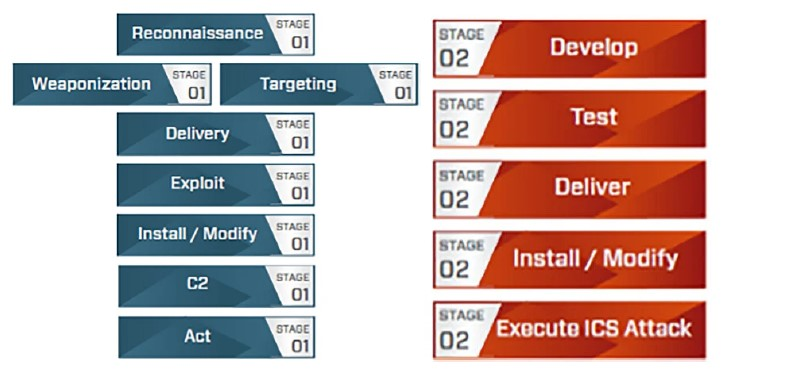
\includegraphics[width=14.5cm]{figure/Figure_2.3.jpg}
\caption{The Industrial Control System Cyber Kill Chain} \label{fig:Figure_2.3.jpg}
\end{figure}

\newpage

\subsection{MITRE ATT\&CK® for ICS}
The MITRE ATT\&CK® for Industrial Control Systems (ICS) framework \cite{ref_report17} serves as a comprehensive knowledge base that categorizes adversary tactics, techniques, and procedures (TTPs) specifically tailored for Operational Technology (OT) environments. As illustrated in the matrix overview in Figure~\ref{fig:Figure_2.4.jpg}, it addresses the unique cyber-physical nature of industrial networks by detailing specific attack stages. Mapping IDS rules to these structured techniques allows defenders to achieve robust, behavior-based threat recognition, rather than solely relying on easily evaded static signatures.

\begin{figure}[htbp]
\centering
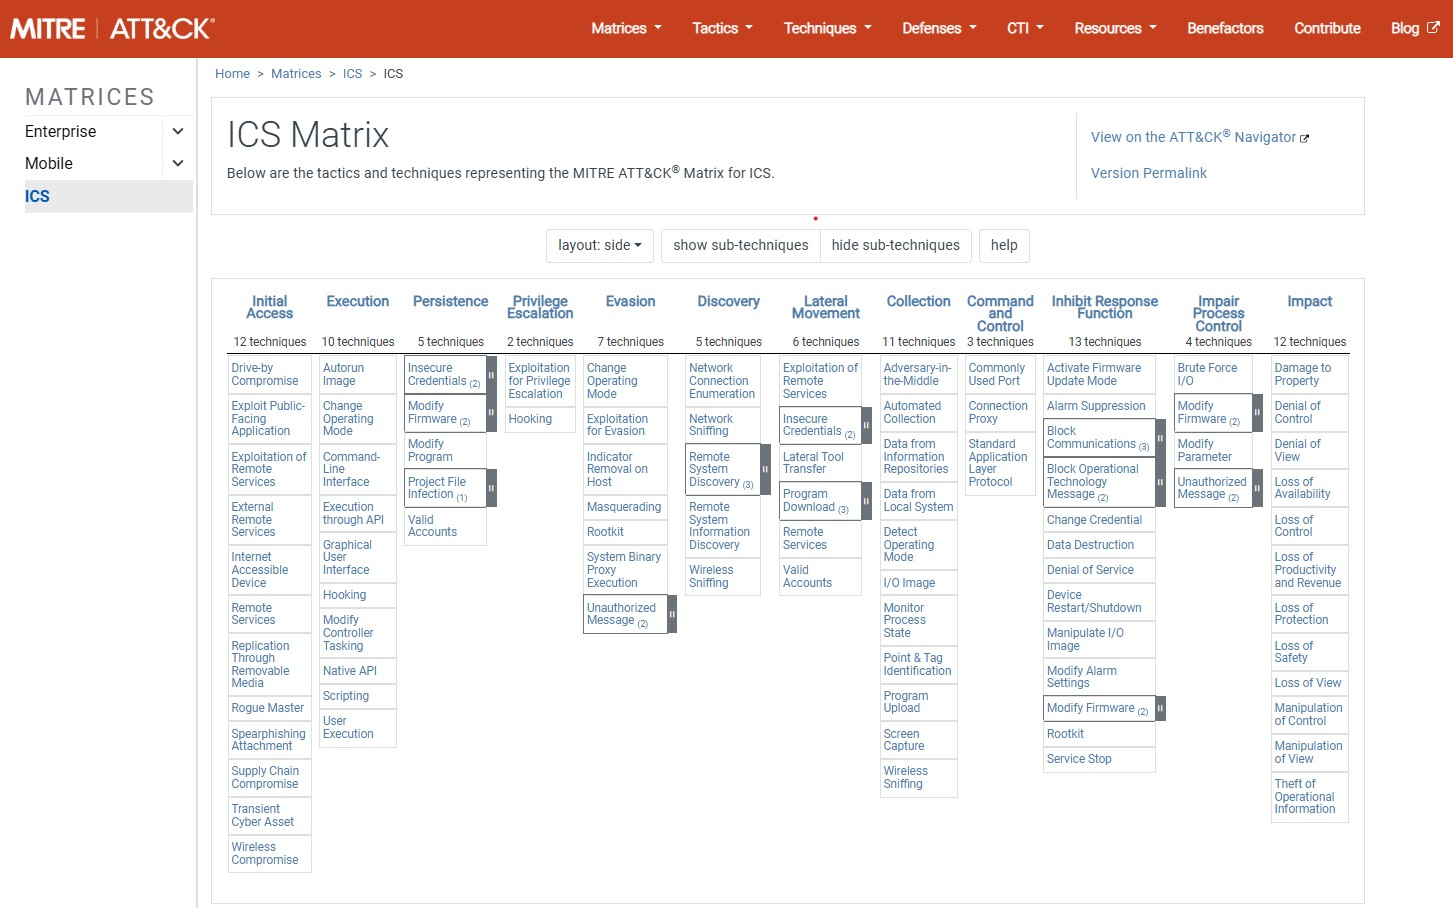
\includegraphics[width=14.5cm]{figure/Figure_2.4.jpg}
\caption{MITRE ATT\&CK® Matrix for ICS} \label{fig:Figure_2.4.jpg}
\end{figure}

\newpage

\section{Deep Packet Inspection (DPI) \& Security Information and Event Management (SIEM)}
To effectively monitor the ICS vulnerabilities and framework requirements mentioned above, deploying appropriate detection and management tools is indispensable. This section introduces the core technologies of our proposed architecture: Deep Packet Inspection (DPI) for precise threat detection at the protocol level, followed by SIEM for centralized monitoring and analysis.

\subsection{Deep Packet Inspection (DPI) and Suricata}
Defending Modbus/TCP can be supported by DPI-based mechanisms \cite{ref_report18}, while granular operational and communication data can further enhance cybersecurity
monitoring in industrial drive environments \cite{ref_report19}. This is particularly important because Modbus/TCP is susceptible to protocol-based attacks, such as reconnaissance,command injection, denial-of-service attacks \cite{ref_report20}.In Figure~\ref{fig:Figure_2.5.png}, the DPI decoding process is clearly shown, allowing the system to identify selected protocol-level anomalies through its advanced application-layer parsing features (e.g., keyword and offset inspection using byte\_test). This approach ensures the effective interception of unauthorized commands and enhances the overall robustness of the detection mechanism.
\begin{figure}[htbp]
\centering
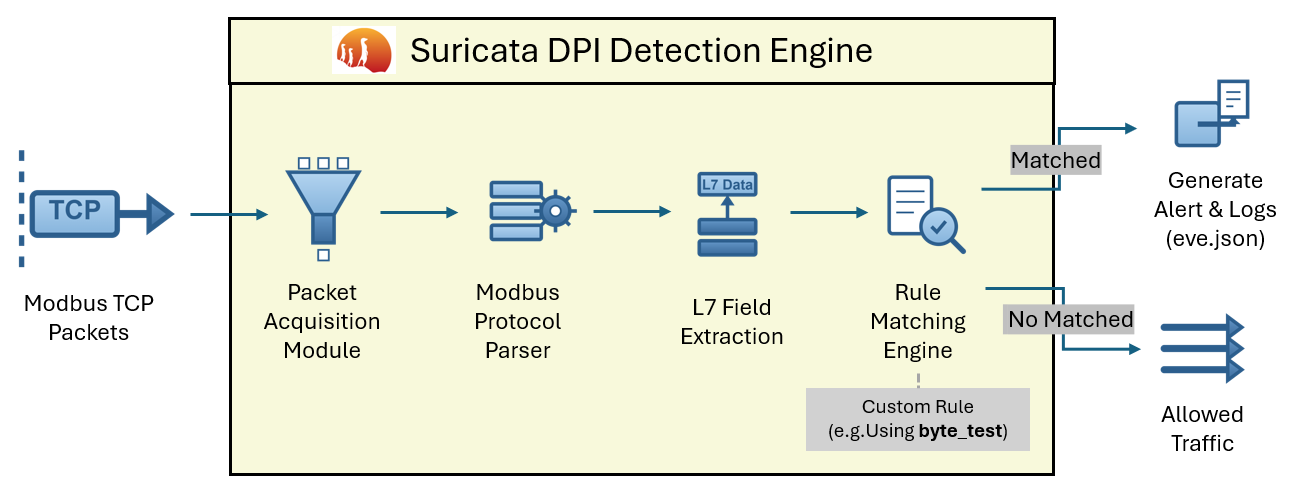
\includegraphics[width=14.5cm]{figure/Figure_2.5.png}
\caption{Suricata DPI Detection Engine} \label{fig:Figure_2.5.png}
\end{figure}

\subsection{Security Information and Event Management (SIEM) Technology and Graylog}
Seamlessly integrating OT data into defense systems is a key strategy \cite{ref_report21}. This enables the SIEM platform to effectively grasp the overall cybersecurity posture \cite{ref_report22}. Furthermore, open-source tools provide cost-effective management solutions \cite{ref_report23}, and their high-performance architecture ensures real-time correlation \cite{ref_report24}. To maintain a simple defense solution and avoid operational blind spots, we adopt Graylog. Graylog pipelines transform raw logs into structured fields for correlation and alerting. More importantly, it provides a real-time alerting mechanism. When an incident occurs, alert information is instantly transmitted to the maintenance personnel's communication devices via Slack, empowering rapid incident response. As illustrated in Figure~\ref{fig:Figure_2.6.png}, combining these threat notifications with intuitive SIEM dashboards not only prevents delayed reactions but also empowers personnel to perform rapid incident response.

\begin{figure}[htbp]
\centering
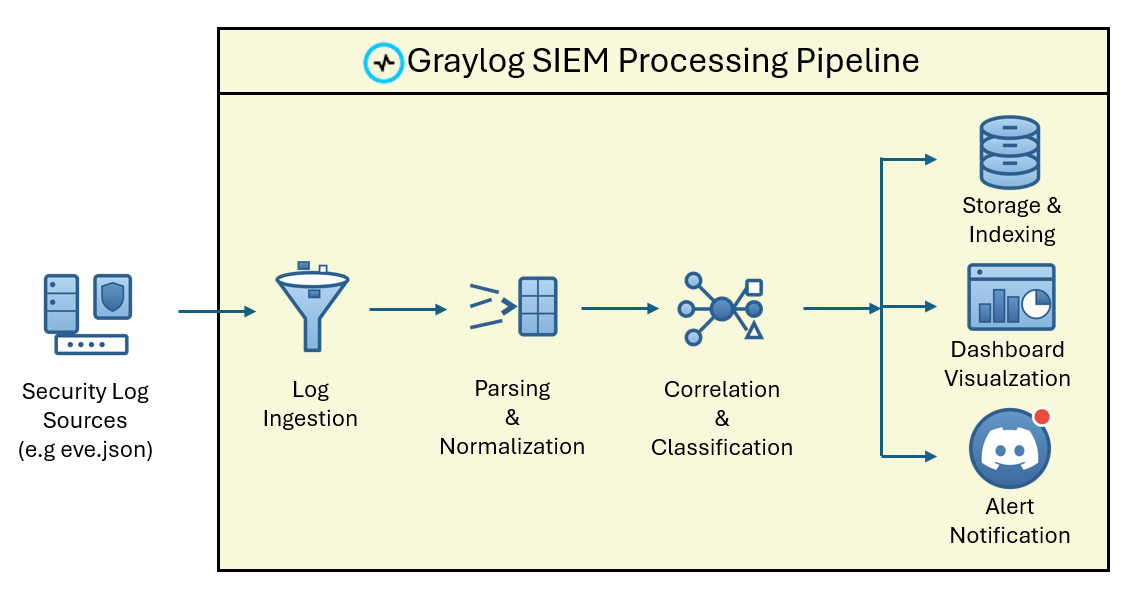
\includegraphics[width=14.5cm]{figure/Figure_2.6.png}
\caption{Graylog SIEM Processing Pipeline} \label{fig:Figure_2.6.png}
\end{figure}

\newpage